\documentclass[12pt,a4paper]{article}

% ================== ENCODING & LANGUAGE ==================
\usepackage[utf8]{inputenc}
\usepackage[T1]{fontenc}
\usepackage[english]{babel}

% ================== FONT ==================
% Using default Computer Modern (guaranteed available)

% ================== PAGE / LAYOUT ==================
\usepackage[top=3cm, bottom=3cm, left=2.5cm, right=2.5cm, headheight=20pt]{geometry}
\usepackage{setspace}
\setstretch{1.15}
\sloppy
\emergencystretch=3em
\setlength{\parskip}{4pt}
\setlength{\parindent}{0pt}

% ================== MATH ==================
\usepackage{amsmath}
\usepackage{amssymb}

% ================== COLORS / GRAPHICS ==================
\usepackage{graphicx}
\usepackage[table]{xcolor}
\usepackage{tikz}
\usetikzlibrary{calc,positioning,arrows.meta}

% ================== FLOATS / LISTS ==================
\usepackage{float}
\usepackage{caption}
\usepackage{enumitem}
\usepackage{multicol}

% ================== BOXES ==================
\usepackage{tcolorbox}
\tcbuselibrary{breakable,skins}

% ================== HEADERS / FOOTERS ==================
\usepackage{fancyhdr}
\usepackage{titlesec}
\usepackage{hyperref}
\usepackage{booktabs}
\usepackage{array}
\usepackage{tabularx}
\usepackage{colortbl}

% ================== COLOR PALETTE ==================
\definecolor{inkblack}{HTML}{1A1A1A}
\definecolor{deepred}{HTML}{8B0000}
\definecolor{darkgray}{HTML}{3A3A3A}
\definecolor{medgray}{HTML}{6B6B6B}
\definecolor{softgray}{HTML}{9A9A9A}
\definecolor{lightgray}{HTML}{E8E8E8}
\definecolor{pagebg}{HTML}{F7F5F2}
\definecolor{boxbg}{HTML}{F9F7F4}
\definecolor{roadblack}{HTML}{1A1A1A}
\definecolor{roadwhite}{HTML}{EDEDED}
\definecolor{donebg}{HTML}{E8F0E8}

\hypersetup{
    colorlinks=true,
    linkcolor=deepred,
    urlcolor=deepred,
}

\titleformat{\section}
  {\normalfont\Large\bfseries\color{deepred}}{\thesection}{1em}{}[\vspace{2pt}{\color{lightgray}\hrule height 0.5pt}]
\titleformat{\subsection}
  {\normalfont\large\bfseries\color{darkgray}}{\thesubsection}{1em}{}

% ================== ROAD PATTERN BORDER ==================
\newcommand{\roadpattern}[1]{%
  \begin{tikzpicture}[remember picture, overlay]
    \pgfmathsetmacro{\blockw}{0.45}%
    \pgfmathsetmacro{\blockh}{0.35}%
    \pgfmathtruncatemacro{\nblocks}{ceil(21.5/\blockw)+1}%
    \foreach \i in {0,...,\nblocks}{%
      \pgfmathtruncatemacro{\parity}{mod(\i,2)}%
      \ifnum#1=0
        \ifnum\parity=0
          \fill[roadblack] ([xshift=\i*\blockw cm]current page.north west)
            rectangle +(\blockw cm, -\blockh cm);
          \fill[roadwhite] ([xshift=\i*\blockw cm, yshift=-\blockh cm]current page.north west)
            rectangle +(\blockw cm, -\blockh cm);
        \else
          \fill[roadwhite] ([xshift=\i*\blockw cm]current page.north west)
            rectangle +(\blockw cm, -\blockh cm);
          \fill[roadblack] ([xshift=\i*\blockw cm, yshift=-\blockh cm]current page.north west)
            rectangle +(\blockw cm, -\blockh cm);
        \fi
      \else
        \ifnum\parity=0
          \fill[roadblack] ([xshift=\i*\blockw cm]current page.south west)
            rectangle +(\blockw cm, \blockh cm);
          \fill[roadwhite] ([xshift=\i*\blockw cm, yshift=\blockh cm]current page.south west)
            rectangle +(\blockw cm, \blockh cm);
        \else
          \fill[roadwhite] ([xshift=\i*\blockw cm]current page.south west)
            rectangle +(\blockw cm, \blockh cm);
          \fill[roadblack] ([xshift=\i*\blockw cm, yshift=\blockh cm]current page.south west)
            rectangle +(\blockw cm, \blockh cm);
        \fi
      \fi
    }%
  \end{tikzpicture}%
}

% ================== HEADERS / FOOTERS ==================
\pagestyle{fancy}
\fancyhf{}
\fancyhead[L]{\small\color{medgray}\textsc{\nouppercase{\leftmark}}}
\fancyhead[R]{%
  \IfFileExists{logo-uir-black.png}{
\includegraphics[height=0.5cm]{logo-uir-black.png}}{\textsc{\small UIR}}%
}
\fancyhead[C]{\roadpattern{0}}
\fancyfoot[C]{\color{medgray}\thepage}
\fancyfoot[L]{\roadpattern{1}}
\renewcommand{\headrulewidth}{0.4pt}
\renewcommand{\headrule}{\hbox to\headwidth{\color{lightgray}\leaders\hrule height \headrulewidth\hfill}}

% ================== CUSTOM BOXES ==================
\newtcolorbox{phasebox}[1][]{
  enhanced, width=\linewidth, before skip=6pt, after skip=10pt,
  colback=boxbg, colframe=deepred, boxrule=1pt, arc=4pt,
  fonttitle=\bfseries\color{white}, colbacktitle=deepred,
  toptitle=3pt, bottomtitle=3pt, #1
}
\newtcolorbox{problembox}[1][]{
  enhanced, width=\linewidth, before skip=6pt, after skip=10pt, breakable,
  colback=white, colframe=darkgray, boxrule=0.8pt, arc=4pt,
  fonttitle=\bfseries\color{white}, colbacktitle=darkgray,
  toptitle=3pt, bottomtitle=3pt, #1
}
\newtcolorbox{enhbox}[1][]{
  enhanced, width=\linewidth, before skip=4pt, after skip=8pt,
  colback=boxbg, colframe=lightgray, boxrule=0.6pt, arc=4pt,
  fonttitle=\bfseries\color{deepred},
  toptitle=3pt, bottomtitle=3pt,
  borderline west={3pt}{0pt}{deepred}, #1
}

% ============================================================
\begin{document}

% ============ TITLE PAGE ============
\begin{titlepage}
    \pagecolor{pagebg}
    \roadpattern{0}
    \centering
    \vspace*{1.5cm}
    \IfFileExists{logo-uir-black.png}{
\includegraphics[height=3.5cm]{logo-uir-black.png}}{\Huge\textbf{UIR}}

    \vspace{0.8cm}
    {\color{deepred}\rule{\textwidth}{2pt}}\\[0.5cm]
    {\Huge\bfseries\color{inkblack} RoadSign}\\[6pt]
    {\huge\bfseries\color{deepred} Project Roadmap}\\[6pt]
    {\large\color{darkgray} Traffic Sign Detection \& Recognition for ADAS}\\[4pt]
    {\color{deepred}\rule{\textwidth}{1pt}}\\[1cm]

    {\Large\color{medgray}\textsc{--- Hermes Vigilia ---}}\\[0.8cm]

    \renewcommand{\arraystretch}{1.4}
    \begin{tabular}{l r}
    Fadwa Bourrich          & 119315 \\
    Abdelmoati Elkoufachy   & 123495 \\
    Zine-elabidine Essabbar & 119351 \\
    \end{tabular}

    \vspace{0.8cm}
    {\color{darkgray}\textbf{Supervised by:} Pr. Najlae Boulajoul}

    \vspace{0.6cm}
    \begin{minipage}{0.45\textwidth}
        \begin{flushleft}
            \textbf{\color{inkblack}Course:}\\
            Advanced Computer Vision\\with Deep Neural Networks
        \end{flushleft}
    \end{minipage}
    \hfill
    \begin{minipage}{0.45\textwidth}
        \begin{flushright}
            \textbf{\color{inkblack}Program:}\\
            5th-year Engineering\\Big Data \& AI
        \end{flushright}
    \end{minipage}

    \vfill
    {\color{medgray}\rule{\textwidth}{0.5pt}}
    \roadpattern{1}
\end{titlepage}
\nopagecolor

% ============================================================
\section*{Project Overview}
% ============================================================

An ADAS equipment maker needs a system that detects and recognises traffic signs from a dashcam feed in real time on embedded hardware. \textbf{RoadSign} builds that system over five weeks using two German benchmarks.

\begin{table}[H]
\centering\small
\renewcommand{\arraystretch}{1.4}
\begin{tabularx}{\textwidth}{l l X c}
\toprule
\textbf{Dataset} & \textbf{Task} & \textbf{Content} & \textbf{Test frozen?} \\
\midrule
GTSDB & Detection       & 900 dashcam images (1360$\times$800\,px) & Yes (300 images) \\
GTSRB & Classification  & 50\,000+ sign crops, 43 classes         & Yes (official set) \\
\bottomrule
\end{tabularx}
\end{table}

\vspace{-4pt}

% --- TIMELINE DIAGRAM ---
\begin{center}
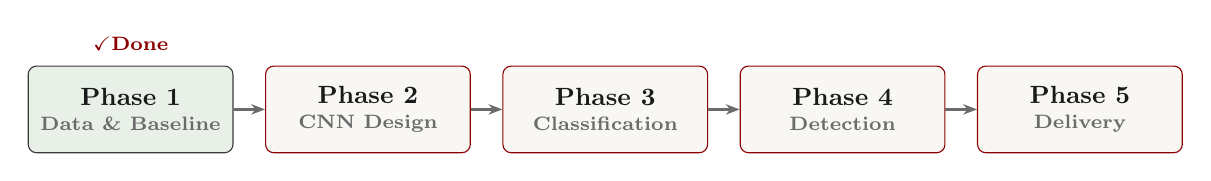
\begin{tikzpicture}[
    phase/.style={draw=deepred, fill=boxbg, rounded corners=3pt,
                  minimum height=1.1cm, minimum width=2.6cm,
                  font=\small\bfseries, text=inkblack, align=center},
    done/.style={phase, fill=donebg, draw=darkgray},
    arr/.style={-{Stealth[length=5pt]}, thick, color=medgray},
]
    \node[done]  (p1) {Phase 1\\[-2pt]\scriptsize\color{medgray}Data \& Baseline};
    \node[phase, right=0.4cm of p1] (p2) {Phase 2\\[-2pt]\scriptsize\color{medgray}CNN Design};
    \node[phase, right=0.4cm of p2] (p3) {Phase 3\\[-2pt]\scriptsize\color{medgray}Classification};
    \node[phase, right=0.4cm of p3] (p4) {Phase 4\\[-2pt]\scriptsize\color{medgray}Detection};
    \node[phase, right=0.4cm of p4] (p5) {Phase 5\\[-2pt]\scriptsize\color{medgray}Delivery};

    \draw[arr] (p1) -- (p2);
    \draw[arr] (p2) -- (p3);
    \draw[arr] (p3) -- (p4);
    \draw[arr] (p4) -- (p5);

    %

    \node[above=2pt of p1, font=\scriptsize\bfseries\color{deepred}] {\checkmark Done};
\end{tikzpicture}
\end{center}

% ============================================================
\section*{Phase 1 : Data Pipeline \& Baseline {\normalsize\color{medgray}\textsc{[completed]}}}
% ============================================================

\begin{phasebox}[title={What We Built}]
\begin{itemize}[leftmargin=1.2em, itemsep=3pt]
  \item \textbf{Data loading \& quality audit.} Parsed all GTSDB annotations. Flagged degenerate boxes, duplicates, out-of-range classes, and unannotated images.
  \item \textbf{Test-set guard.} \texttt{assert\_not\_test()} raises an error if any script tries to access a frozen test image. Covered by 3 unit tests.
  \item \textbf{Leak-free splits.} GTSDB split by blocks of 20 consecutive frames; GTSRB split by physical sign track. Saved as JSON, never recomputed.
  \item \textbf{YOLO export.} Annotations converted to Ultralytics layout in two variants: 43-class and 1-class (for detect-then-classify).
  \item \textbf{Classical baseline.} HSV colour segmentation + contour filtering for detection; HOG features + linear SVM for classification.
  \item \textbf{Synthetic augmentation module.} Copy-paste pipeline that places training sign crops onto training backgrounds with feathered blending and random transforms.
  \item \textbf{22 unit tests} covering boxes, splits, guard, baseline, and augmentation.
\end{itemize}
\end{phasebox}

\vspace{4pt}

% --- PHASE 1 RESULTS TABLE ---
\begin{table}[H]
\centering\small
\renewcommand{\arraystretch}{1.3}
\caption{Phase 1 results at a glance.}
\begin{tabular}{l c | l c}
\toprule
\multicolumn{2}{c|}{\textbf{Data}} & \multicolumn{2}{c}{\textbf{Baseline (validation)}} \\
\midrule
GTSDB train images       & 600                & Detection recall @IoU$\geq$0.5 & 39.6\%  \\
GTSDB annotations        & 506                & Classification accuracy         & 74.3\%  \\
Classes present           & 40 / 43            & Speed                           & 83 FPS  \\
\midrule
GTSRB train images        & 39\,209           & \multicolumn{2}{c}{\textbf{Splits}} \\
GTSRB classes             & 43 / 43           & GTSDB (train / val) & 480 / 120 \\
Imbalance ratio           & 10.7$\times$      & GTSRB (train / val) & 31\,379 / 7\,830 \\
\bottomrule
\end{tabular}
\end{table}

% --- PROBLEMS BOX ---
\begin{problembox}[title={Problems Encountered \& Fixes}]

\textbf{1. GTSDB on Kaggle stored in YOLO format, not the expected \texttt{gt.txt}.}\\
Labels were per-image \texttt{.txt} files with normalised \texttt{class cx cy w h}, while our pipeline expected the original semicolon-delimited annotation file.\\
\textit{Fix:} Wrote \texttt{prepare\_kaggle.py} to reverse-convert YOLO labels back to pixel-coordinate \texttt{gt.txt}.

\medskip\noindent{\color{lightgray}\hrule height 0.5pt}\medskip

\textbf{2. GTSRB track split returned an empty validation set.}\\
Kaggle names files \texttt{CLASS\_TRACK\_FRAME.png} (3 parts). Our splitter assumed the original 2-part naming and grabbed the class prefix instead of the track ID, collapsing all files into one ``track.''\\
\textit{Fix:} Detect the 3-part format and use \texttt{parts[1]} as the track ID when \texttt{len(parts) >= 3}.

\medskip\noindent{\color{lightgray}\hrule height 0.5pt}\medskip

\textbf{3. Baseline precision returned \texttt{NaN}.}\\
Images where the detector found zero candidates produced \texttt{NaN} precision. \texttt{np.mean} then propagated it to the final average.\\
\textit{Fix:} Used \texttt{np.nanmean} and filtered out \texttt{NaN} values before aggregation.

\end{problembox}

% ============================================================
\section*{Phase 2 : CNN Architecture Design}
% ============================================================

\begin{phasebox}[title={Ch.~2--3: Hand-Computed Architecture Table}]
\begin{itemize}[leftmargin=1.2em, itemsep=3pt]
  \item Design a CNN for 32$\times$32 sign classification into 43 classes.
  \item Hand-compute every layer's output dimensions using:
  \[
    O = \left\lfloor \frac{I + 2P - K_{\mathrm{eff}}}{S} \right\rfloor + 1 \qquad K_{\mathrm{eff}} = d(K-1)+1
  \]
  \item Build a full architecture table: layer type, kernel, stride, padding, output shape, and parameter count.
  \item Verify hand computations match PyTorch's \texttt{model.parameters()} exactly.
  \item Justify design choices: depth vs.\ receptive field vs.\ parameter budget for a 32$\times$32 input.
\end{itemize}
\end{phasebox}

% ============================================================
\section*{Phase 3 : Classification Experiments}
% ============================================================

\begin{phasebox}[title={EF2: Scratch CNN vs.\ Pretrained}]
\begin{itemize}[leftmargin=1.2em, itemsep=3pt]
  \item Train the designed CNN from scratch on the GTSRB training split.
  \item Fine-tune a pretrained backbone (e.g.\ ResNet-18) on the same split.
  \item Run controlled experiments changing one factor at a time: learning rate, data augmentation, architecture depth.
  \item Log configuration, seed, and git commit hash for every run.
  \item Compare accuracy, convergence speed, and parameter count.
\end{itemize}
\end{phasebox}

% --- EXPERIMENT PLAN TABLE ---
\begin{table}[H]
\centering\small
\renewcommand{\arraystretch}{1.3}
\caption{Planned one-factor-at-a-time experiment grid.}
\begin{tabularx}{\textwidth}{l l X}
\toprule
\textbf{Factor} & \textbf{Values} & \textbf{Goal} \\
\midrule
Learning rate    & 1e-2, 1e-3, 1e-4   & Find sweet spot for convergence \\
Augmentation     & None, flip+rotate, full pipeline & Measure regularisation benefit \\
Architecture     & Scratch CNN, ResNet-18 & Compare capacity vs.\ efficiency \\
Synthetic data   & Off, on (A2)       & Quantify copy-paste augmentation gain \\
\bottomrule
\end{tabularx}
\end{table}

% ============================================================
\section*{Phase 4 : Detection \& Integration}
% ============================================================

\begin{phasebox}[title={EF3 / EF4 / EF5: Detection + Post-Processing + Demo}]
\begin{itemize}[leftmargin=1.2em, itemsep=3pt]
  \item Train two detectors on GTSDB: \textbf{YOLOv8} (single-stage) and \textbf{Faster R-CNN} (two-stage).
  \item Apply from-scratch post-processing: IoU computation, greedy NMS, class-aware NMS.
  \item Evaluate: mAP@0.5, recall, F1 per class, and inference speed (ms/image, FPS).
  \item Plug in enhancements \textbf{A1} (detect-then-classify) and \textbf{A2} (synthetic augmentation).
  \item Build a web demo (\textbf{A6}): upload a dashcam image, see bounding boxes and class labels.
\end{itemize}
\end{phasebox}

% --- DETECTION PIPELINE DIAGRAM ---
\begin{center}
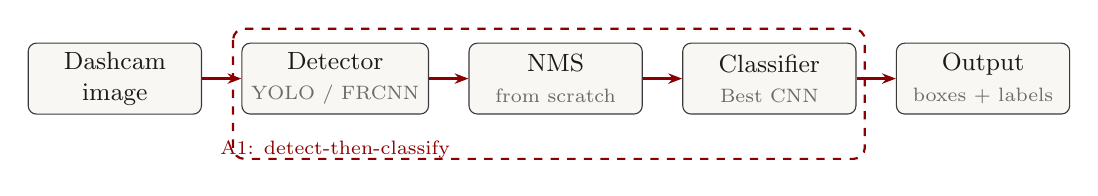
\begin{tikzpicture}[
    block/.style={draw=darkgray, fill=boxbg, rounded corners=3pt,
                  minimum height=0.9cm, minimum width=2.2cm,
                  font=\small, text=inkblack, align=center},
    arr/.style={-{Stealth[length=5pt]}, thick, color=deepred},
]
    \node[block] (img) {Dashcam\\image};
    \node[block, right=0.5cm of img] (det) {Detector\\{\scriptsize\color{medgray}YOLO / FRCNN}};
    \node[block, right=0.5cm of det] (nms) {NMS\\{\scriptsize\color{medgray}from scratch}};
    \node[block, right=0.5cm of nms] (cls) {Classifier\\{\scriptsize\color{medgray}Best CNN}};
    \node[block, right=0.5cm of cls] (out) {Output\\{\scriptsize\color{medgray}boxes + labels}};

    \draw[arr] (img) -- (det);
    \draw[arr] (det) -- (nms);
    \draw[arr] (nms) -- (cls);
    \draw[arr] (cls) -- (out);

    \node[below=6pt of det, font=\scriptsize\color{deepred}] {A1: detect-then-classify};
    \draw[deepred, dashed, thick, rounded corners=4pt]
        ($(det.north west)+(-3pt,5pt)$) rectangle ($(cls.south east)+(3pt,-16pt)$);
\end{tikzpicture}
\end{center}

% ============================================================
\section*{Phase 5 : Final Evaluation \& Delivery}
% ============================================================

\begin{phasebox}[title={Robustness, Quantisation, Defence}]
\begin{itemize}[leftmargin=1.2em, itemsep=3pt]
  \item Export models to ONNX and quantise to INT8 (\textbf{A3}). Benchmark latency and accuracy drop.
  \item Run robustness analysis: performance on small signs ($\leq$32\,px), rare classes, and low-contrast subsets.
  \item Complete the conformity table with EF/ENF status for every course criterion.
  \item Execute the one-shot evaluation on frozen test sets; run once, report final numbers.
  \item Finalise report and prepare defence presentation.
\end{itemize}
\end{phasebox}

% ============================================================
\section*{Enhancements}
% ============================================================

\begin{enhbox}[title={A1 : Detect-Then-Classify Pipeline}]
A class-agnostic detector (1-class YOLO, trained on the \texttt{1cls} export) proposes sign regions. Each crop is classified by the best CNN from Phase~3. This decouples localisation from recognition, letting each model specialise and making it easy to upgrade either independently.
\end{enhbox}

\begin{enhbox}[title={A2 : Synthetic Data Augmentation}]
GTSDB has only 600 training images and 3 classes with zero examples. The copy-paste module pastes real GTSRB crops onto training backgrounds with feathered masks, random brightness shifts, and motion blur. An ablation study will measure the actual gain.
\end{enhbox}

\begin{enhbox}[title={A3 : ONNX / INT8 Quantisation Benchmark}]
The final models are exported to ONNX, then quantised to INT8. We measure inference latency, throughput (FPS), and accuracy degradation compared to full-precision. This directly answers whether the system is deployable on embedded hardware.
\end{enhbox}

\begin{enhbox}[title={A6 : Web Demo (EF5)}]
A Gradio or Streamlit interface where the user uploads a dashcam image and sees the full pipeline output: detected sign regions with bounding boxes and predicted class labels overlaid.
\end{enhbox}

% --- CONFORMITY OVERVIEW TABLE ---
\vspace{6pt}
\begin{table}[H]
\centering\small
\renewcommand{\arraystretch}{1.25}
\caption{Conformity overview : course requirements mapped to phases.}
\begin{tabularx}{\textwidth}{l X c c}
\toprule
\textbf{ID} & \textbf{Requirement} & \textbf{Phase} & \textbf{Status} \\
\midrule
EF1  & Data pipeline, anomaly report, splits         & 1 & \textbf{\color{deepred}\checkmark} \\
EF2  & Classification (scratch vs.\ pretrained)       & 3 & -- \\
EF3  & Detection (YOLO vs.\ Faster R-CNN)             & 4 & -- \\
EF4  & Post-processing (NMS, JSON output)             & 4 & -- \\
EF5  & Demonstrator (web demo)                        & 4 & -- \\
\midrule
ENF1 & mAP, recall metrics                            & 4 & -- \\
ENF2 & Speed (ms/image, FPS)                          & 4 & -- \\
ENF3 & Model size (params, MB)                        & 5 & -- \\
ENF4 & Robustness subsets                             & 5 & -- \\
ENF5 & Evaluation integrity (test guard)              & 1 & \textbf{\color{deepred}\checkmark} \\
ENF6 & Reproducibility (seeds, configs, splits)       & 1 & \textbf{\color{deepred}\checkmark} \\
\midrule
A1   & Detect-then-classify pipeline                  & 4 & -- \\
A2   & Copy-paste synthetic data                      & 4 & \textit{module ready} \\
A3   & ONNX / INT8 benchmark                          & 5 & -- \\
A6   & Web demo                                       & 4 & -- \\
\bottomrule
\end{tabularx}
\end{table}

\end{document}
